% append.tex
%
% Predrag               jun 20 2006
% $Author$ $Date$

\appendix

\PublicPrivate{%
        }{% switch to Private:

\section{\KSe\ according to Evangelos}
\label{ap:rpo}

The \KSe\ % (KSe)
reads:
 \beq
  u_t=(u^2)_x-u_{xx}- u_{xxxx} \, ,
  \label{eq:KS}
 \eeq

 We assume periodic boundary conditions on the $x\in [0,2\pi \tilde{L}]$
 interval:
 \beq
   u(x+2\pi\tilde{L},t)=u(x,t) \, ,
 \eeq
 which allows a Fourier series expansion:
 \beq
  u(x,t)=\sum_{k=-\infty}^{+\infty} a_k (t) e^{ i k x / \tilde{L}} \, .
  \label{eq:Fourier}
 \eeq
 Since $u(x,t)$ is real,
 \beq
  a_{k}=a^*_{-k} \, .
  \label{eq:a*}
 \eeq
 Substituting \refeq{eq:Fourier} into \refeq{eq:KS} we get:
 \beq
  \dot{a}_k=(k/\tildeL)^2\left(1-(1/\tildeL)^2 k^2\right)a_k
        + i (k/\tildeL)  \sum_{m=-\infty}^{+\infty}a_m a_{k-m} \, .
  \label{eq:Fcoef}
 \eeq

 From \refeq{eq:Fcoef} we notice that $\dot{a}_0=0$ and thus $a_0$ is an integral
 of the equations or, from \refeq{eq:Fourier}, the average of the solution $\int dx u(x,t)$
 is a constant. Due to galilean invariance we may set $a_0=0$ without loss of generality
 and we only have to compute $a_k$'s with $k\geq 1$. % Explain this in detail somewhere.

 Truncating the infinite tower of equations by setting $a_k=0$ for $k>d$, using the identity $a_{-k}=a^*_k$ and splitting the
 resulting equations into real and imaginary part by setting $a_k=b_k+i c_k$, we have

 \bea
  \dot{b}_k & = & \left(\frac{k}{\tildeL}\right)^2\left(1- \left(k/\tildeL\right)^2 \right)b_k  \continue
    & & - \frac{k}{\tildeL} \left(\sum_{m=1}^{k-1}c_m b_{k-m}+\sum_{m=k+1}^{N}c_m b_{m-k}
                    -\sum_{m=1}^{N-k}c_m b_{k+m} \right)  \continue
    & & - \frac{k}{\tildeL} \left(\sum_{m=1}^{k-1}b_m c_{k-m}-\sum_{m=k+1}^{N}b_m c_{m-k}
                    +\sum_{m=1}^{N-k}b_m c_{k+m} \right)
  \label{eq:tmp:b-Trunc}
 \eea
 \bea
   \dot{c}_k & = & \left(\frac{k}{\tildeL}\right)^2\left(1- \left(k/\tildeL\right)^2 \right)c_k  \continue
    & & - \frac{k}{\tildeL}\left( \sum_{m=1}^{k-1}c_m c_{k-m}-\sum_{m=k+1}^{N}c_m c_{m-k}
                    -\sum_{m=1}^{N-k}c_m c_{k+m} \right)    \continue
    & & + \frac{k}{\tildeL} \left(\sum_{m=1}^{k-1}b_m b_{k-m}+\sum_{m=k+1}^{N}b_m b_{m-k}
                    +\sum_{m=1}^{N-k}b_m b_{k+m} \right)
   \label{eq:tmp:c-Trunc}
 \eea
 where now only terms $c_{k},b_{k}$ with $0<k<d$ appear. Observe
 \beq
    \sum_{m=1}^{N-k}c_m b_{k+m} = \sum_{m=k+1}^{N}b_m c_{m-k}\,,
 \eeq
 \etc and thus \refeq{eq:tmp:b-Trunc} and \refeq{eq:tmp:c-Trunc} simplify to
  \bea
  \dot{b}_k & = & \left(\frac{k}{\tildeL}\right)^2\left(1- \left(k/\tildeL\right)^2 \right)b_k  \continue
    & & - \frac{k}{\tildeL} \left(\sum_{m=1}^{k-1}c_m b_{k-m}-2\sum_{m=1}^{N-k}c_m b_{k+m} \right)  \continue
    & & - \frac{k}{\tildeL} \left(\sum_{m=1}^{k-1}b_m c_{k-m}+2\sum_{m=1}^{N-k}b_m c_{k+m} \right)
  \label{eq:b-Trunc}
 \eea
 \bea
   \dot{c}_k & = & \left(\frac{k}{\tildeL}\right)^2\left(1- \left(k/\tildeL\right)^2 \right)c_k  \continue
    & & - \frac{k}{\tildeL}\left( \sum_{m=1}^{k-1}c_m c_{k-m}-2\sum_{m=1}^{N-k}c_m c_{k+m} \right)  \continue
    & &  +\frac{k}{\tildeL}\left( \sum_{m=1}^{k-1}b_m b_{k-m}+2\sum_{m=1}^{N-k}b_m b_{k+m} \right)\,.
   \label{eq:c-Trunc}
 \eea

 We begin by calculating the matrix of variations $A_{ij} \equiv \frac{\partial v_i(x)}{\partial x_j}$ for the antisymmetric
 subspace for which $b_k=0, c_{-k}=-c_{k}$ and thus
 \beq
       \dot{c}_k =  \left(\frac{k}{\tildeL}\right)^2\left(1- \left(k/\tildeL\right)^2 \right)c_k
            - \frac{k}{\tildeL}\left( \sum_{m=1}^{k-1}c_m c_{k-m}
                            -2\sum_{m=1}^{N-k}c_m c_{k+m} \right)   \,.
 \eeq

 Then
 \bea
    \frac{\partial \dot{c}_k}{\partial c_{j}}  =
        \left(\frac{k}{\tildeL}\right)^2\left(1- \left(k/\tildeL\right)^2 \right) \delta_{kj}
            - \frac{k}{\tildeL}\frac{\partial}{\partial c_j}\left( \sum_{m=1}^{k-1}c_m c_{k-m}-2\sum_{m=1}^{N-k}c_m c_{k+m} \right) \,.
 \eea
 Concider the second term:
 \bea
    - \frac{k}{\tildeL}\frac{\partial}{\partial c_j}\left( \sum_{m=1}^{k-1}c_m c_{k-m}-2\sum_{m=1}^{N-k}c_m c_{k+m} \right) & = &
        - \frac{k}{\tildeL} \sum_{m=1}^{k-1} \left(\delta_{m,j} c_{k-m}+c_m \delta_{k-m,j} \right) \continue
                        & & + 2 \frac{k}{\tildeL}\sum_{m=1}^{N-k} \left(\delta_{m,j} c_{k+m}+c_m \delta_{k+m,j}\right)
 \eea
 We need to consider two cases separately:
 \begin{itemize}
    \item $k\leq j$
        \bea
             -\frac{k}{\tildeL}\frac{\partial}{\partial c_j}\left( \sum_{m=1}^{k-1}c_m c_{k-m}-2\sum_{m=1}^{N-k}c_m c_{k+m} \right) & = &
                    -\frac{k}{\tildeL}( 0+0 ) + 2\frac{k}{\tildeL} (c_{k+j} + c_{j-k}) \continue
                & = &   2 \frac{k}{\tildeL} (c_{k+j}-c_{k-j})
        \eea
    \item $k > j$
        \bea
             -\frac{k}{\tildeL}\frac{\partial}{\partial c_j}\left( \sum_{m=1}^{k-1}c_m c_{k-m}-2\sum_{m=1}^{N-k}c_m c_{k+m} \right) & = &
                    -\frac{k}{\tildeL}(c_{k-j} + c_{k-j} ) + 2\frac{k}{\tildeL} (c_{k+j}  + 0 ) \continue
                & = &  2 \frac{k}{\tildeL} (c_{k+j}-c_{k-j})
        \eea
 \end{itemize}
 and thus
 \beq
    \frac{\partial \dot{c}_k}{\partial c_{j}} =  \left(\frac{k}{\tildeL}\right)^2\left(1- \left(k/\tildeL\right)^2 \right)\delta_{kj} + 2 \frac{k}{\tildeL} (c_{k+j}-c_{k-j})
 \eeq

 For the case of the full space we need to consider the four matrices $\frac{\partial \dot{b}_k}{\partial b_j},\frac{\partial \dot{b}_k}{\partial c_j},\frac{\partial \dot{c}_k}{\partial b_j},\frac{\partial \dot{c}_k}{\partial c_j}$. Following the above procedure
 \beq
    \frac{\partial \dot{c}_k}{\partial b_{j}} =  2 \frac{k}{\tildeL} ( b_{k+j}+b_{k-j} )\,,
 \eeq
 \beq
    \frac{\partial \dot{b}_k}{\partial b_{j}} =  \left(\frac{k}{\tildeL}\right)^2\left(1- \left(k/\tildeL\right)^2 \right)\delta_{kj} - 2 \frac{k}{\tildeL} (c_{k+j} + c_{k-j}) \,,
 \eeq
 \beq
    \frac{\partial \dot{b}_k}{\partial c_{j}} = 2 \frac{k}{\tildeL} (b_{k+j}-b_{k-j}) \,.
 \eeq


\section{\KS\ according to Ruslan}
The \KSe\ has a slightly different form:
\begin{equation}
  u_t=-{\textstyle\frac{1}{2}}(u^2)_x-u_{xx}- u_{xxxx} \, ,
\end{equation}
which can be reduced to Eq.~(\ref{eq:KS}) by the transformation $u
\rightarrow -2u$.

The \KSe\ in terms of Fourier modes:
\begin{equation}
  \hat{u}_k \equiv {\cal F}[u]_k = \frac{1}{L}\int_0^L u(x,t) e^{-ikx/\tilde{L}}dx\,,
  \qquad u(x,t) \equiv {\cal F}^{-1}[\hat{u}] = \sum_{k\in{\mathbb Z}} \hat{u}_k e^{ikx/\tilde{L}}
\end{equation}
 is given by
\begin{equation}
  \dot{\hat{u}}_k =[(k/\tildeL)^2-(k/\tildeL)^4]\hat{u}_k -
  \frac{ik}{2\tilde{L}}{\cal F}[({\cal F}^{-1}[\hat{u}])^2]_k\,.
\end{equation}
Since $u$ is real, the Fourier modes are related by $\hat{u}_{-k} =
\hat{u}^\ast_k$.

The above system is truncated as follows: The Fourier transform
${\cal F}$ is replaced by its discrete equivalent
\begin{equation}
  a_k \equiv {\cal F}_N[u]_k = \sum_{n = 0}^{N-1} u(x_n)
  e^{-ikx_n/\tilde{L}}\,,\qquad u(x_n) \equiv {\cal F}_N^{-1}[a]_n
  = \frac{1}{N}\sum_{k = 0}^{N-1} a_k e^{ikx_n/\tilde{L}}\,,
\end{equation}
where $x_n = 2\pi\tilde{L}n/N$ and $a_{N-k} = a^\ast_k$.  Since $a_0
= 0$ due to galilean invariance and setting $a_{N/2} = 0$ (assuming
$N$ is even), the number of independent variables in the truncated
system is $N-2$.  The truncated system looks as follows:
\begin{equation}
  \dot{a}_k =[(k/\tildeL)^2-(k/\tildeL)^4]a_k -
  \frac{ik}{2\tilde{L}}{\cal F}_N[({\cal F}_N^{-1}[a])^2]_k\,.
\end{equation}
with $k = 1,\ldots,N/2-1$, although in the Fourier transform we need
to use $a_k$ over the full range of $k$ values from 0 to $N-1$.

The discrete Fourier transform ${\cal F}_N$ can be computed by FFT.
In Fortran and C, the routine {\tt REALFT} from Numerical Recipes
can be used.  In Matlab, it is more convenient to use complex
variables for $a_k$.  Note that Matlab function {\tt fft} is, in
fact, the inverse Fourier Transform.

To derive the equation for the matrix of variations, I use the fact
that ${\cal F}_N$ is a linear operator.  Since we need to
differentiate separately with respect to the real and imaginary
components of $a_k$, I use the notation $a_k = b_{2k-1} + ib_{2k}$.
\begin{equation}
  \frac{\partial \dot{a}_k}{\partial b_j} =
  [(k/\tildeL)^2-(k/\tildeL)^4]\delta_{kj} -
  \frac{ik}{\tilde{L}}{\cal F}_N[{\cal F}_N^{-1}[a]\cdot{\cal
  F}_N^{-1}[\delta_{kj}]]\,,\quad j = 1,\ldots,N-2
\end{equation}
where the dot indicates componentwise product, and the inverse
Fourier transform is applied separately to each column of
$\delta_{kj}$. Here, $\delta_{kj}$ is not a standard Kronecker
delta, but a complex valued $N\times N-2$ matrix:
\begin{equation}
  \delta_{kj} = \left(
  \begin{array}{ccccc}
  0 &  0 & 0 &  0 &\cdots\\
  1 &  i & 0 &  0 &\cdots\\
  0 &  0 & 1 &  i &\cdots\\
\multicolumn{5}{c}\dotfill \\
  0 &  0 & 0 &  0 &\cdots\\
\multicolumn{5}{c}\dotfill \\
  0 &  0 & 1 & -i &\cdots\\
  1 & -i & 0 &  0 &\cdots\\
  \end{array}  \right),
\end{equation}
with index $k$ running from 0 to $N-1$.  I admit, the notations are
a bit stretched here, but I find them convenient when coding this
equation using FFT.

\section{Tales from the Literature}

\subsection{\KSe\ according to Kuramoto and Sivashinsky}

The original form in which \KSe was derived (in $1-D$) was (up to scaling factors):
\beq
	y_t=-y_{xxxx}-y_{xx}-\frac{1}{2}y_x^2\,,
	\label{eq:KSeOR}
\eeq
with periodic boundary conditions in the $(0,L)$ interval. The equation we are using
differs in the nonlinear term:
\beq 
	u_t=-u_{xxxx}-u_{xx}-uu_x\,.
	\label{eq:KSeAP}
\eeq
It can be obtained from \refeq{eq:KSeOR} by setting $u=y_x$. The two equations are used interchangeably
and referred to as \KSe. The authors of \refref{TsveTri89} state that the solutions of the two equations
differ considerably despite the simple way they are related. 

\subsection{\KSe according to Greene and Kim}

Greene and Kim \refref{ksgreene88} use the following form of \KSe:
\beq
	y_t=-4y_{xxxx}-\alpha\left(y_{xx}+\frac{1}{2}y_x^2-\frac{1}{4\pi}\int_0^{2\pi}y_x^2\ dx\right)\,,
	\label{eq:KSeGreeneKim}
\eeq
where $\alpha$ the bifurcation parameter and periodic boundary conditions are assumed in the $(0,2\pi)$
interval. To see its relation to our form of the equation, first take the derivative of \refeq{eq:KSeGreeneKim}
with respect to $x$ and then make the substitution $y_x=u$ to obtain
\beq
	u_t=-4u_{xxxx}-\alpha\left(u_{xx}+uu_x\right)\,.
\eeq
Rescale according to
\beq
	\tilde{x}=\frac{\alpha^{1/2}}{2} x
	\label{eq:GKxScale}
\eeq
\beq
	\tilde{t}=\frac{\alpha^2}{4} t
\eeq
\beq
	\tilde{u}=\frac{2}{a^{1/2}} u
\eeq
to obtain \refeq{eq:KSeAP}. From \refeq{eq:GKxScale} we see that our control parameter $\tilde{L}=L/2\pi$ is connected
to $\alpha$ through $\frac{\alpha^{1/2}}{2}$. Thus our system size $L=22.0$ corresponds to $\alpha=49.0395$.

%%%%%%%%%%%%%%%%%%%%%%%%%%%%%%%%%%%%%%%%%%%%%%%%%%%%%%%%%%%%%%%%
\begin{figure}[t]
	% \vspace*{-5pt}
\centering
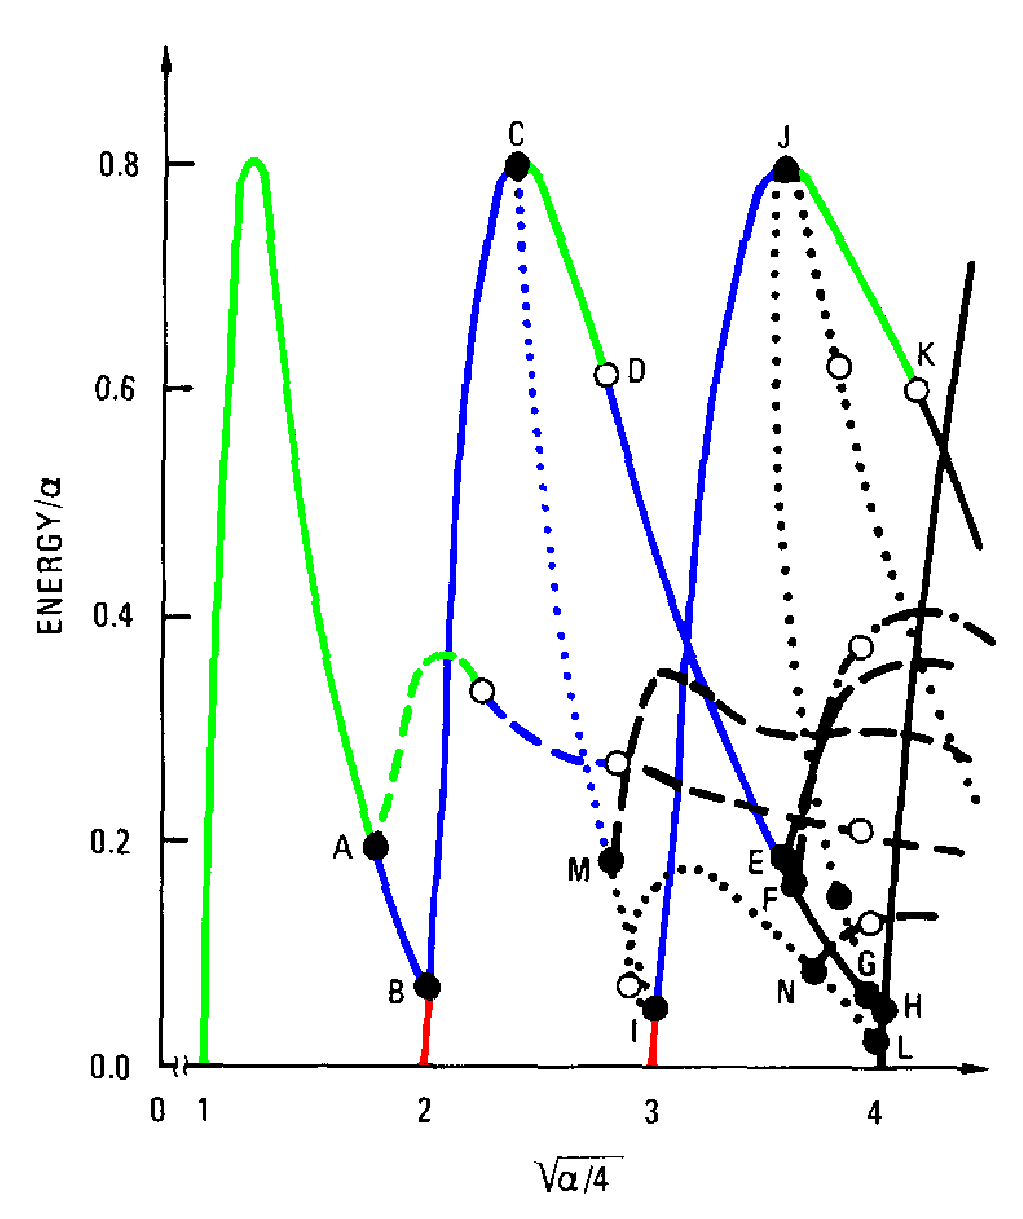
\includegraphics[width=0.5\textwidth]{figs/GreeneKimBifColor.eps}
	% \vspace*{-5pt}
\caption{
	{\small
The energy of steady states as a function of the bifurcation
parameter a. The solid curves are N-cell solutions,
dotted curves are for GLMRT, the dash-dotted curve is for the
giant states, and dashed curves are for the propagating solutions.
Open circles are for Hopf bifurcation. From \refref{ksgreene88}. Here
we've color-coded the branches to reflect the number of unstable
eigenvalues (or complex pairs). Red: 2 unstable eigenvalues, Blue: 1
unstable eigenvalue, Green: stable. Regions that could not be
resolved with the help of \refref{ksgreene88} or are of no interest
to our present purposes have been left black.
        } %end \small
        }
\label{fig:GreeneKim}
	% \vspace*{-5pt}
\end{figure}
%%%%%%%%%%%%%%%%%%%%%%%%%%%%%%%%%%%%%%%%%%%%%%%%%%%%%%%%%%%%%%%%%%

Greene and Kim systematically study the steady states of \KSe\ and their bifurcations, extending the work of
previous authors, \refrefs{Mks86,laquey74}. We review their bifurcation diagram, \reffig{fig:GreeneKim}, up to
the system size that we use. They define the energy as
\beq
	E=\frac{1}{2\pi}\int_0^{2\pi}y_x^2\, dx\,.
\eeq
Since $u=y_x$ we have from \refeq{eq:stdks} that $c\sim E$. 

For small $\alpha$ the only equilibrium state of the system is the trivial state, $y(x,t)=0$, which is
stable for $\tilde{L}=(a/4)^{1/2}<1$. At $\tilde{L}=N$, with $N$ integer, the $N$'th harmonic becomes unstable and
the trivial state bifurcates to the so called $N$-cell states. These states contain only the multiples of the $N$'th
harmonic, i.e. only the components $a_N,a_{2N},...$ in our notation. 
Moreover, the $N$-cell states are found to be symmetric (in our case, since $u=y_x$ they will be
antisymmetric). In general Greene and Kim show that symmetric solutions are not traveling. 
At point $A$ in \reffig{fig:GreeneKim} the $1$-cell state loses stability and bifurcates to a stable, 
asymetric traveling wave solution, which later on becomes unstable through a Hopf bifurcation. 

At $\tilde{L}=(a/4)^{1/2}=2$ the system has become large enough that a $2$-cell steady state appears. At point $B$
in \reffig{fig:GreeneKim} the $1$-cell branch merges to the $2$-cell branch. In general each $N$-cell branch merges to the corresponding $2N$-cell branch.

At point $C$ in \reffig{fig:GreeneKim} the $2$-cell state bifurcates to a type of equilibrium solution
found by La Quey, Mahajan, Rutherford and Tang, \refref{laquey74} and generalized by Greene and Kim who refer to them as GLMRT equilibria. GLMRT solutions are symmetric (u(x) is antisymmetric) and can be roughly described as long-wave distorted $N$-cell states.

The last type of solution identified in \refref{ksgreene88} appears at point $F$ in \reffig{fig:GreeneKim} and is termed
giant state. because its amplitude grows as the system size increases.

According to the bifurcation diagram \reffig{fig:GreeneKim}, at the point that corresponds to our system size $\tilde{L}=\frac{\alpha^{1/2}}{2}=3.501$ the steady states we should expect are the $2$- and $3$-cell states ($\EQV{2}$ and $\EQV{3}$ respectivelly), the GLMRT state that bifurcates from a $3$-cell state at point $I$ ($\EQV{1}$) and the traveling waves that belong to the branches starting at points $A$ ($\REQV{\pm}{1}$) and $M$ (not identified yet).
 
        }% end \PublicPrivate
